\chapter{Tackling Difficult Problems: Positive Semidefinite Matrices}

With all the computing power available today, you’d think no problem would be too difficult to tackle. But that’s not so. There is a category of problems called NP (nondeterministic polynomial time) whose solution is easy to verify but whose computation is difficult to perform because there is no straightforward algorithm and any brute-force method would take too much time. For these problems, all we can do is to develop an efficient algorithm that can find a solution in a reasonable amount of time. While the solution might not be the most optimal, the goal is to find the best solution possible in a short time. 

As you learn more about optimization techniques, you’ll come across many efficiency algorithms that have been used throughout the years. In the 1990’s, the field of optimization changed with the discovery that algorithms based on  semidefinite positive matrices can achieve a higher efficiency than seen in the past. Today, there is an entire field of programming—Semidefinite Programming—based on the use of semidefinite positive matrices.

First we’ll take a look at what some of the NP problems are. Then we’ll describe the intuition behind semidefinite positive matrices. We’ll take a look at one NP problem and then introduce the python module to use for solving these problems. 

\section{NP Problems}

In the world of mathematics, easy problems are referred to as P, or polynomial time, problems. In simple terms, this means the problem can be solved quickly and it’s easy to verify that the solution is correct. Addition, subtraction, division, multiplication, square roots, matrix-vector multiplication, are just a few examples. But NP problems, as stated in the introduction, can’t be computed in any reasonable amount of time but solutions are usually easy to verify. The game of Sudoku is one such example. It’s easy to verify a correct solution, but writing a generalized algorithm to solve any Sudoku game is an NP problem. 

NP problems show up in many other situations, such as:
\begin{itemize}
\item Designing  robust communication networks
\item Scheduling tasks without conflicts
\item Managing supply chains
\item Detecting patterns in biological networks
\item Figuring out subgroups in social networks
\item Predicting the structure of proteins
\end{itemize}

For each of these situations think of large scale problems for which there are many variables. A cloud computing company that provides AI services to thousands of clients must be able to schedule tasks efficiently and in a timely manner as well as manage the power needed for the computers and cooling the data center. Supply chain management is crucial to figuring out how to pick up, transport, and distribute goods to help provide disaster relief. Understanding protein structure is important for designing drugs that can tackle specific conditions. All we can do for each of these situations is to find an optimal solution, but not the definitive solution.

\section{A Past Approach: Minimizing Errors in Neural Networks}

When neural networks were first being developed to recognize things (faces, letters, music, and so on), the goal was to calculate weights between network nodes that would minimize the recognition error. The error space could be visualized as a surface of valleys and hills. The lowest point would have the least error. The idea behind the iterative weight calculations for training the network was to descend down the gradient until reaching the low point. Without getting into the mathematics, you can see by looking at this figure that there are two valleys. Some neural network training resulted in ending at a low point, but not the lowest point. Wouldn’t it be great if you could formulate an optimization problem so that you’d be guaranteed to land at the lowest point? That's where semidefinite programming can help.

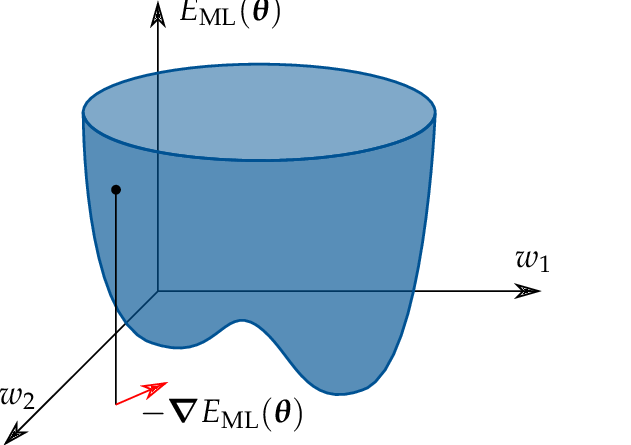
\includegraphics[width=0.5\textwidth]{neuralnet-error-function.png}

\section{Positive Definite and Semidefinite Matrices}

Unlike matrices that are defined by their content (such as identity matrix, zero matrix, and diagonal matrix) positive definite and semidefinite matrices are characterized by the result they produce. They have an analog in the scalar world, so let's first look at that. Let's take the scalars $a$ and $b$ and treat them as vectors. $ab$ is then the dot product. If $a >0$, then $ab$ will take on the sign of $b$. If $a < 0$, then $ab$ will have the opposite sign of $b$. If you look at this graphically, you can see that in the first case $ab$ stays on the same side of the origin, but in the second case, $ab$ flips

For $a = [2], b = [4]$ 

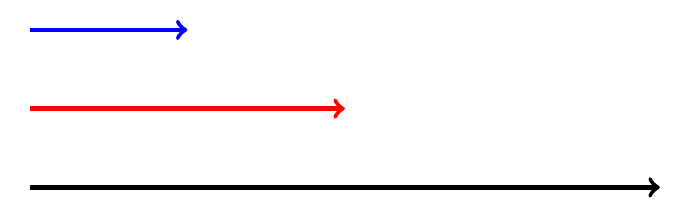
\begin{tikzpicture}
\draw[blue, ultra thick,->] (0,1) -- (2,1);
\draw[red, ultra thick,->] (0,0) -- (4,0);
\draw[black, ultra thick,->] (0,-1) -- (8,-1);
\end{tikzpicture}

For $a = [3], b = [-4]$. the result of multiplication flips a to the other side of the graph. 

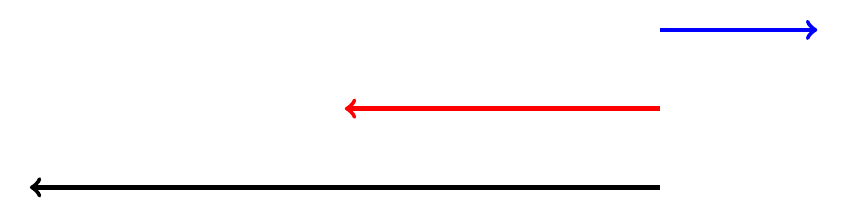
\begin{tikzpicture}
\draw[blue, ultra thick,->] (0,1) -- (2,1);
\draw[red, ultra thick,->] (0,0) -- (-4,0);
\draw[black, ultra thick,->] (0,-1) -- (-8,-1);
\end{tikzpicture}

The notion of “staying on the same side” is positive definite. The notion of flipping is negative definite. Positive definite means that $x > 0$, so the result is a positive number. Positive semidefinite means that $x >= 0$, so the result is a non-negative number. 

If you can formulate a problem as a positive semidefinite matrix, then you automatically constrain the result to the “same side.”  This constraint results in higher algorithmic efficiency.

Let's look at the formal definition:

A matrix is positive definite if, and only if:
$$x^{T}Ax > 0, x,  x \neq 0$$

A matrix is positive semidefinite, if, and only if:
$$x^{T}Ax \geq 0$$

Further, a positive semidefinite matrix had an important property. Its eigenvalues are $\geq 0$. The eigenvalues of a positive definite matrix  are $> 0$.

Take the triplet $(a, b, c)$ and the symmetric matrix:
$$
\begin{bmatrix}
 1  & a & b  \\
 a  & 1 & c  \\
 b  & c & 1  \\
\end{bmatrix}
\geq 0
$$
For what values of $a, b, c$ is this matrix positive semidefinite? If you iterate through all possible combinations of a,b,c and then compute the eigenvalues for each matrix, you'll find that some (like $0,0,0$) result in a postive semidefinite matrix and some (like $2, 2, 2 $) are not positive semidefinite. If you plot the set of triplets that result in a semidefinite matrix, you'll see an elliptope. It's this shape that guarantees an optimal solution.

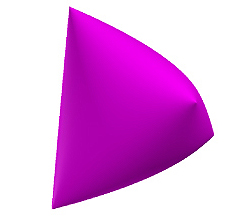
\includegraphics[width=0.5\textwidth]{elliptope.jpg}

\section{Identifying and Constructing a Positive Semidefinite Matrix}
In the last section, you saw that being symmetric does not guarantee a positive semidefinite matrix. You also saw that a matrix of positive values does not guarantee a positive semidefinite matrix. The only way to check for positive semidefinite is to calculate the eigenvalues, which you learned in a previous workbook.

A surefire way to construct a positive semidefinite matrix is:
$$AA^{T}$$

\begin{Exercise}[title={Figuring out if a matrix is positive semidefinite}, label=pos-matrix-01]
Is this matrix positive definite? Show your work.
$$
\begin{bmatrix}
 2  & 2 \\
 2  & 0 \\
\end{bmatrix}
$$
\end{Exercise}

\begin{Answer}[ref=pos-matrix-01]
Yes. It's eigenvalues are $$2,2$$
\end{Answer}
  
\begin{Exercise}[title={Creating a positive semidefinite matrix}, label=pos-matrix-02]
Using any 3 by 3 matrix, create a positive semidefinite matrix.Then show it is positive semidefinite by calculating its eigenvalues.  You can either compute this by hand or using python.  In either case, show your work.
\end{Exercise}

\begin{Answer}[ref=pos-matrix-02]
The answer depends on the 3 by 3 matrix you chose.
\end{Answer}

\section{The Max Cut Problem}
A famous NP problem is Max Cut. Given a graph of interconnected nodes, cut the graph to create two sets of nodes, such that the cut goes through as many edges as possible. (You can't cut an edge more than once.) Max Cut is important for binary classification in machine learning, circuit design, statistical physics, and more. There is no algorithm that will provide an exact solution. If you could find one, you'd be eligible to win a huge prize from the Clay Mathematics Institute. Instead, you'll see how to approximate a solution to this  problem using a positive semidefinite matrix and a technique developed by mathematicians Michel Goemans and David Williamson. 

You won't see all the complete details here as this section is meant to be a quick introduction to how you can apply positive semidefinite matrices. 

Take this simple graph of five nodes and six edges. Each node in the graph will take on one of two values (1 or -1)to show which set they fall into after a cut is made. For any two connected nodes, $x_i*x_j = 1$ if $x_i = x_j$ and $-1$ otherwise.

If you randomly assign $1$ and $-1$ to the nodes, the chance of making the max cut is $0.5$. By using semidefinite programming you can achieve an algorithmic efficiency of $0.87$. 

The Goemans-Williamson technique can be used for any optimization problem where the variables take on the values of $1$ and $-1$.

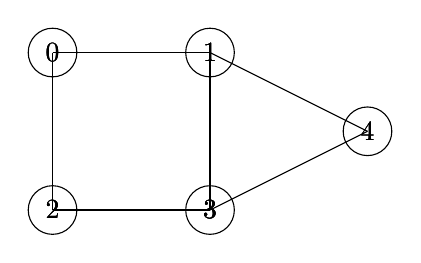
\begin{tikzpicture}
     \node[circle, draw= black] (node 0) {0};
     \node[circle, draw=black, xshift=2cm, at=(node 0)] (node 1) {1};
     \node[circle, draw=black, yshift= -2cm, at=(node 0)] (node 2) {2};
     \node[circle, draw=black, xshift=2cm, yshift= -2cm, at=(node 0)] (node 3) {3};
     \node[circle, draw=black, xshift=4cm, yshift= -1cm, at=(node 0)] (node 4) {4};
     \draw (0,0) node {0} -- (2,0) node {1};
     \draw (0,0) node {0} -- (0,-2) node {2};
     \draw (0,-2) node {2} -- (2,-2) node {3};
     \draw (2,0) node {1} -- (2,-2) node {3};
     \draw (2,0) node {1} -- (4,-1) node {4};
     \draw (2,-2) node {3} -- (4,-1) node {4};   
\end{tikzpicture}

As a list of edges the graph is:

$$ edges = [(0,1),
        (0,2),
        (1,3),
        (1,4),
        (2,3),
        (3,4)] $$
The optimization problem can be formulated as:
$$
Max\sum_{edges(i,j)}{}\frac{1 - x_{i}x_{j}}{2}
$$
for
$$
 x_{i}\in \{ -1,1 \}
$$

BUT instead of allowing $x_{i}$ to be scalar, Goemans-Williamson defines $x_{i}$ as unit vectors.

$$
 x_{i}\in R^n, \left\| x_{i}=1  \right\
$$

and that makes the optimization equation:
$$
Max\sum_{edges(i,j)}{}\frac{1 - x_{i}^{T}x_{j}}{2}
$$
It's this "relaxation" that gets us to a semidefinite matrix, because we can now rewrite the problem as a positive semidefinite matrix:
$$
X = \left[ x_{i}^{T}x_{j} \right]_{i,j}
$$
Python has a module for solving optimization problems. Using this, you'll get an optimum matrix, but to get the unit vectors, you'll need to take the square root of the matrix. 
$$
X = \left[ x_{1}...x_{1n} \right]\left[ x_{1}...x_{1n} \right]^{T}
$$
Next we need to go from unit vectors to scalars, a process called rounding.
$$
x^{i}\in R^n \to x^{i}\in \{ -1,1 \}
$$
Goemans-Williamson leveraged the fact that the end point of a unit vector is on a sphere. They generated a random plane to bisect the sphere. A vector on one side of the plane is assigned the value of $1$ and a vector on the other side a value of $-1$.

You can then assign the scalar values to the nodes and make the cut accordingly. This particular cut will be 5, as shown.

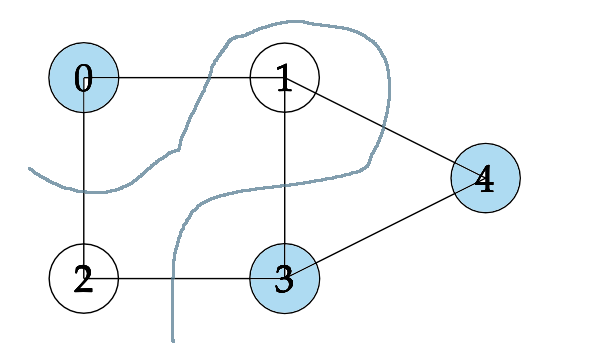
\includegraphics[width=0.5\textwidth]{max-cut.png}

\section{The Max Cut Problem Solved in Python}
\begin{Verbatim}       
# MaxCut Problem
import numpy as np
import scipy 
from scipy.linalg import sqrtm
# cvxpy is a python module for solving optimization problems
import cvxpy as cp

# define the edges of the graph
edges = [(0,1),
        (0,2),
        (1,3),
        (1,4),
        (2,3),
        (3,4)]

#  Declare the matrix X to be positive semidefinite
X = cp.Variable((5,5),symmetric=True)
constraints = [X >> 0]

# Set diagonals to 1 to get unit vectors
constraints += [
    X[i,i] == 1 for i in range(5)
]

# Set the objective function
objective = sum(05.*(1 - X[i,j]) for (i,j)in edges)

# Set up the problem to maximize using the objective function and
# keeping within the set constraints
prob = cp.Problem(cp.Maximize(objective), constraints)

# Returns a positive semidefinite matrix
print(prob.solve())

# To get the vectors take square root of the matrix
x = sqrtm(X.value)

# Generate a random hyperplane
u = np.random.randn(5) # normal to random hyperplane

# Pick values according to which side of the hyperplane the vectors are on
x = np.sign(x @ u)  
      
\end{Verbatim}










